\documentclass[14pt,a4paper]{extarticle}
\usepackage[left=2cm, right=2cm, top=1.5cm, bottom=3cm]{geometry}
% подключаем пакеты
\usepackage[utf8]{inputenc} % кодировка
\usepackage[english, russian]{babel} % русский язык
\usepackage{amsmath} % математическая мода
\usepackage{amssymb} % математическая мода
\usepackage{graphics} % картинки
\usepackage{float}
\usepackage{graphicx,xcolor} % картинки
\usepackage{cite} % пакет для цитирования
%\setcitestyle{authoryear,open={(},close={)}}
\usepackage{lscape} % разваричивает текст под альбомную страницу
\usepackage{caption}
\usepackage{subcaption}
\usepackage{float}
\captionsetup[figure]{font=small}
\usepackage{indentfirst}            %отступ у первой красной строки
\usepackage{hyperref} % для навигации в файле
\usepackage{overpic} % позволяет делать подписи на рисунке
\usepackage{multirow} % позволяет объединять ячейки в таблицах
\usepackage{siunitx}
\setcounter{tocdepth}{2} %%where n is the level, starting with 0 (chapters only)

\newenvironment{localsize}[1]
{%
  \clearpage
  \let\orignewcommand\newcommand
  \let\newcommand\renewcommand
  \makeatletter
  \input{bk#1.clo}%
  \makeatother
  \let\newcommand\orignewcommand
}
{%
  \clearpage
}

\graphicspath{ {./images/} {./images/logo/} }  %место где TeX будет искть рисунки

%Новые команды
\newcommand{\const}{\operatorname{const} }
\newcommand{\sign}{\operatorname{sign} }
\newcommand{\kv}[1]{«{#1}»}


\begin{document}
\pagestyle{plain}
\clearpage
\input titlepageFKI.tex % Титул ФКИ
\newpage
\tableofcontents
\newpage
\section{Введение}
\input introduction.tex
\section{Литературный обзор}
\input literary_review.tex
\section{Постановка проблем и методик}
\input problems.tex
%\section{Описание идеи}
%\input description.tex

\section{Ход выполнения работы}
\input applying.tex
\section{Анализ результатов. Экспериментальная оценка точности}
\input discussion.tex
\section{Заключение}
\input conclusion.tex
\section{Приложение}
\subsection{Приложение 1. Демонстрация установки}\label{sec:application1}
\begin{figure}[H]
    \centering
    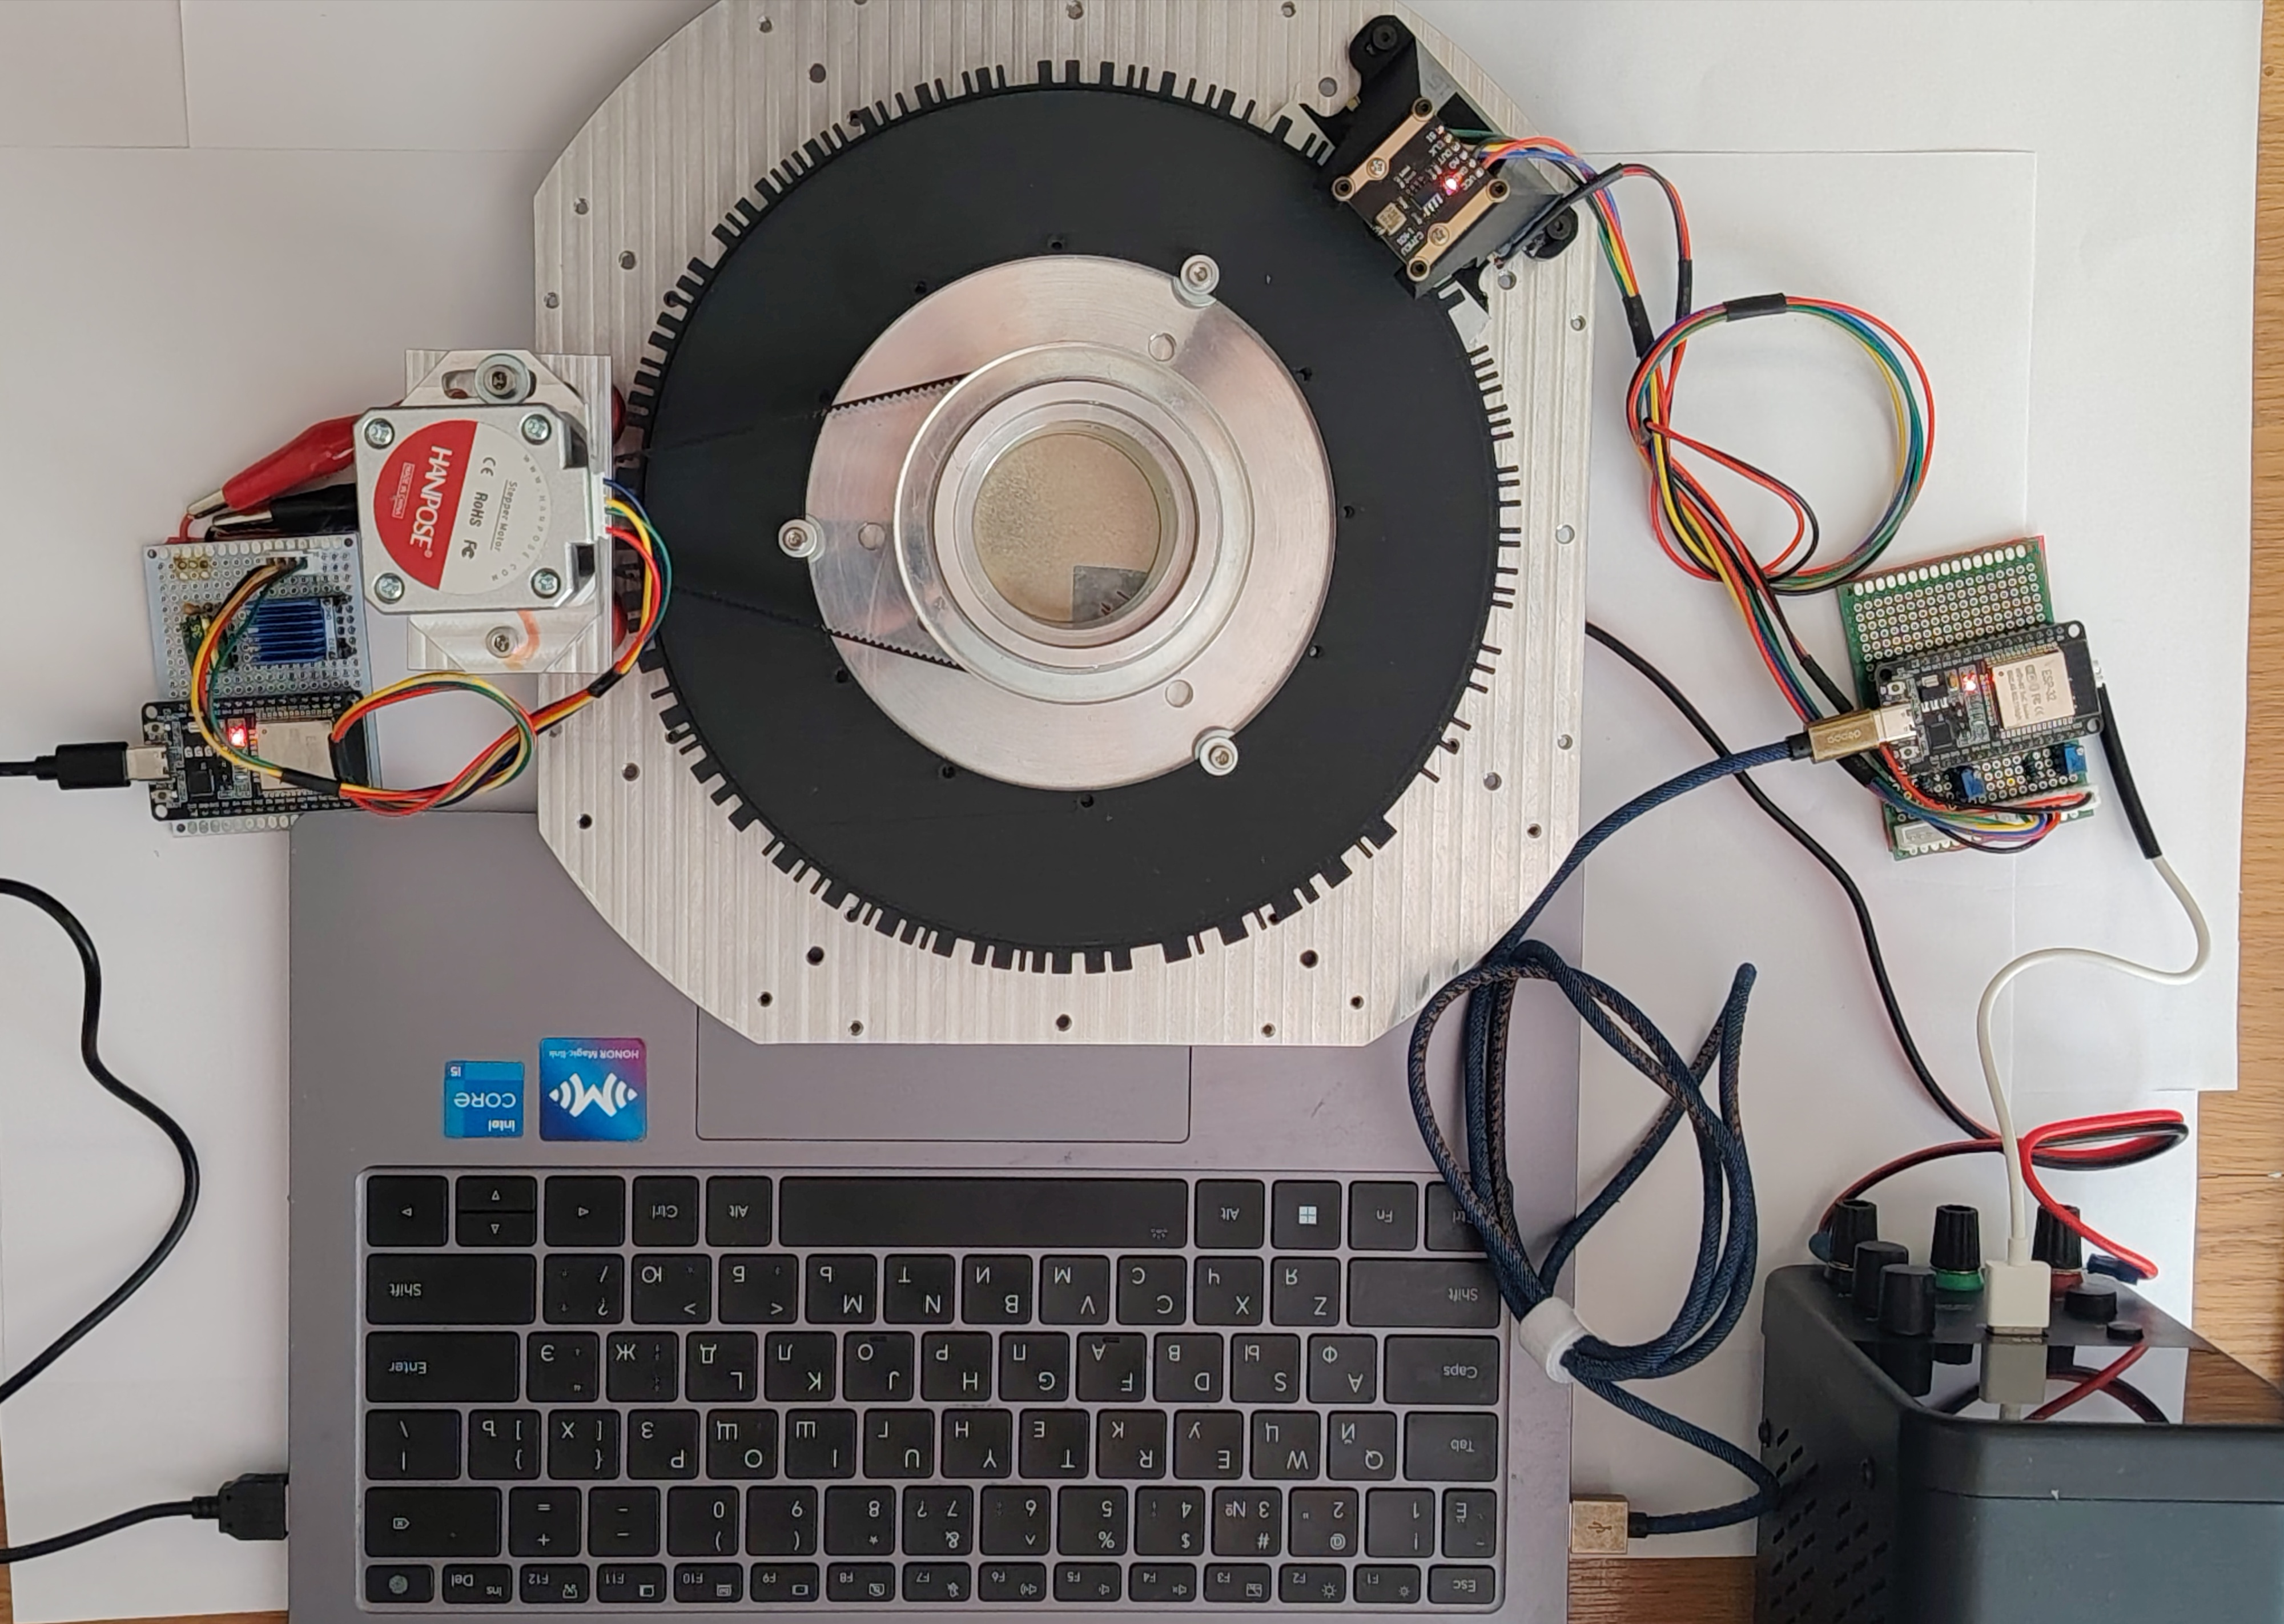
\includegraphics[width=1.2\linewidth, angle=90]{images/установка матовый.jpg}
    \caption{Фото установки (одна головка и компьютер)}
\end{figure}
\begin{figure}[H]
    \centering
    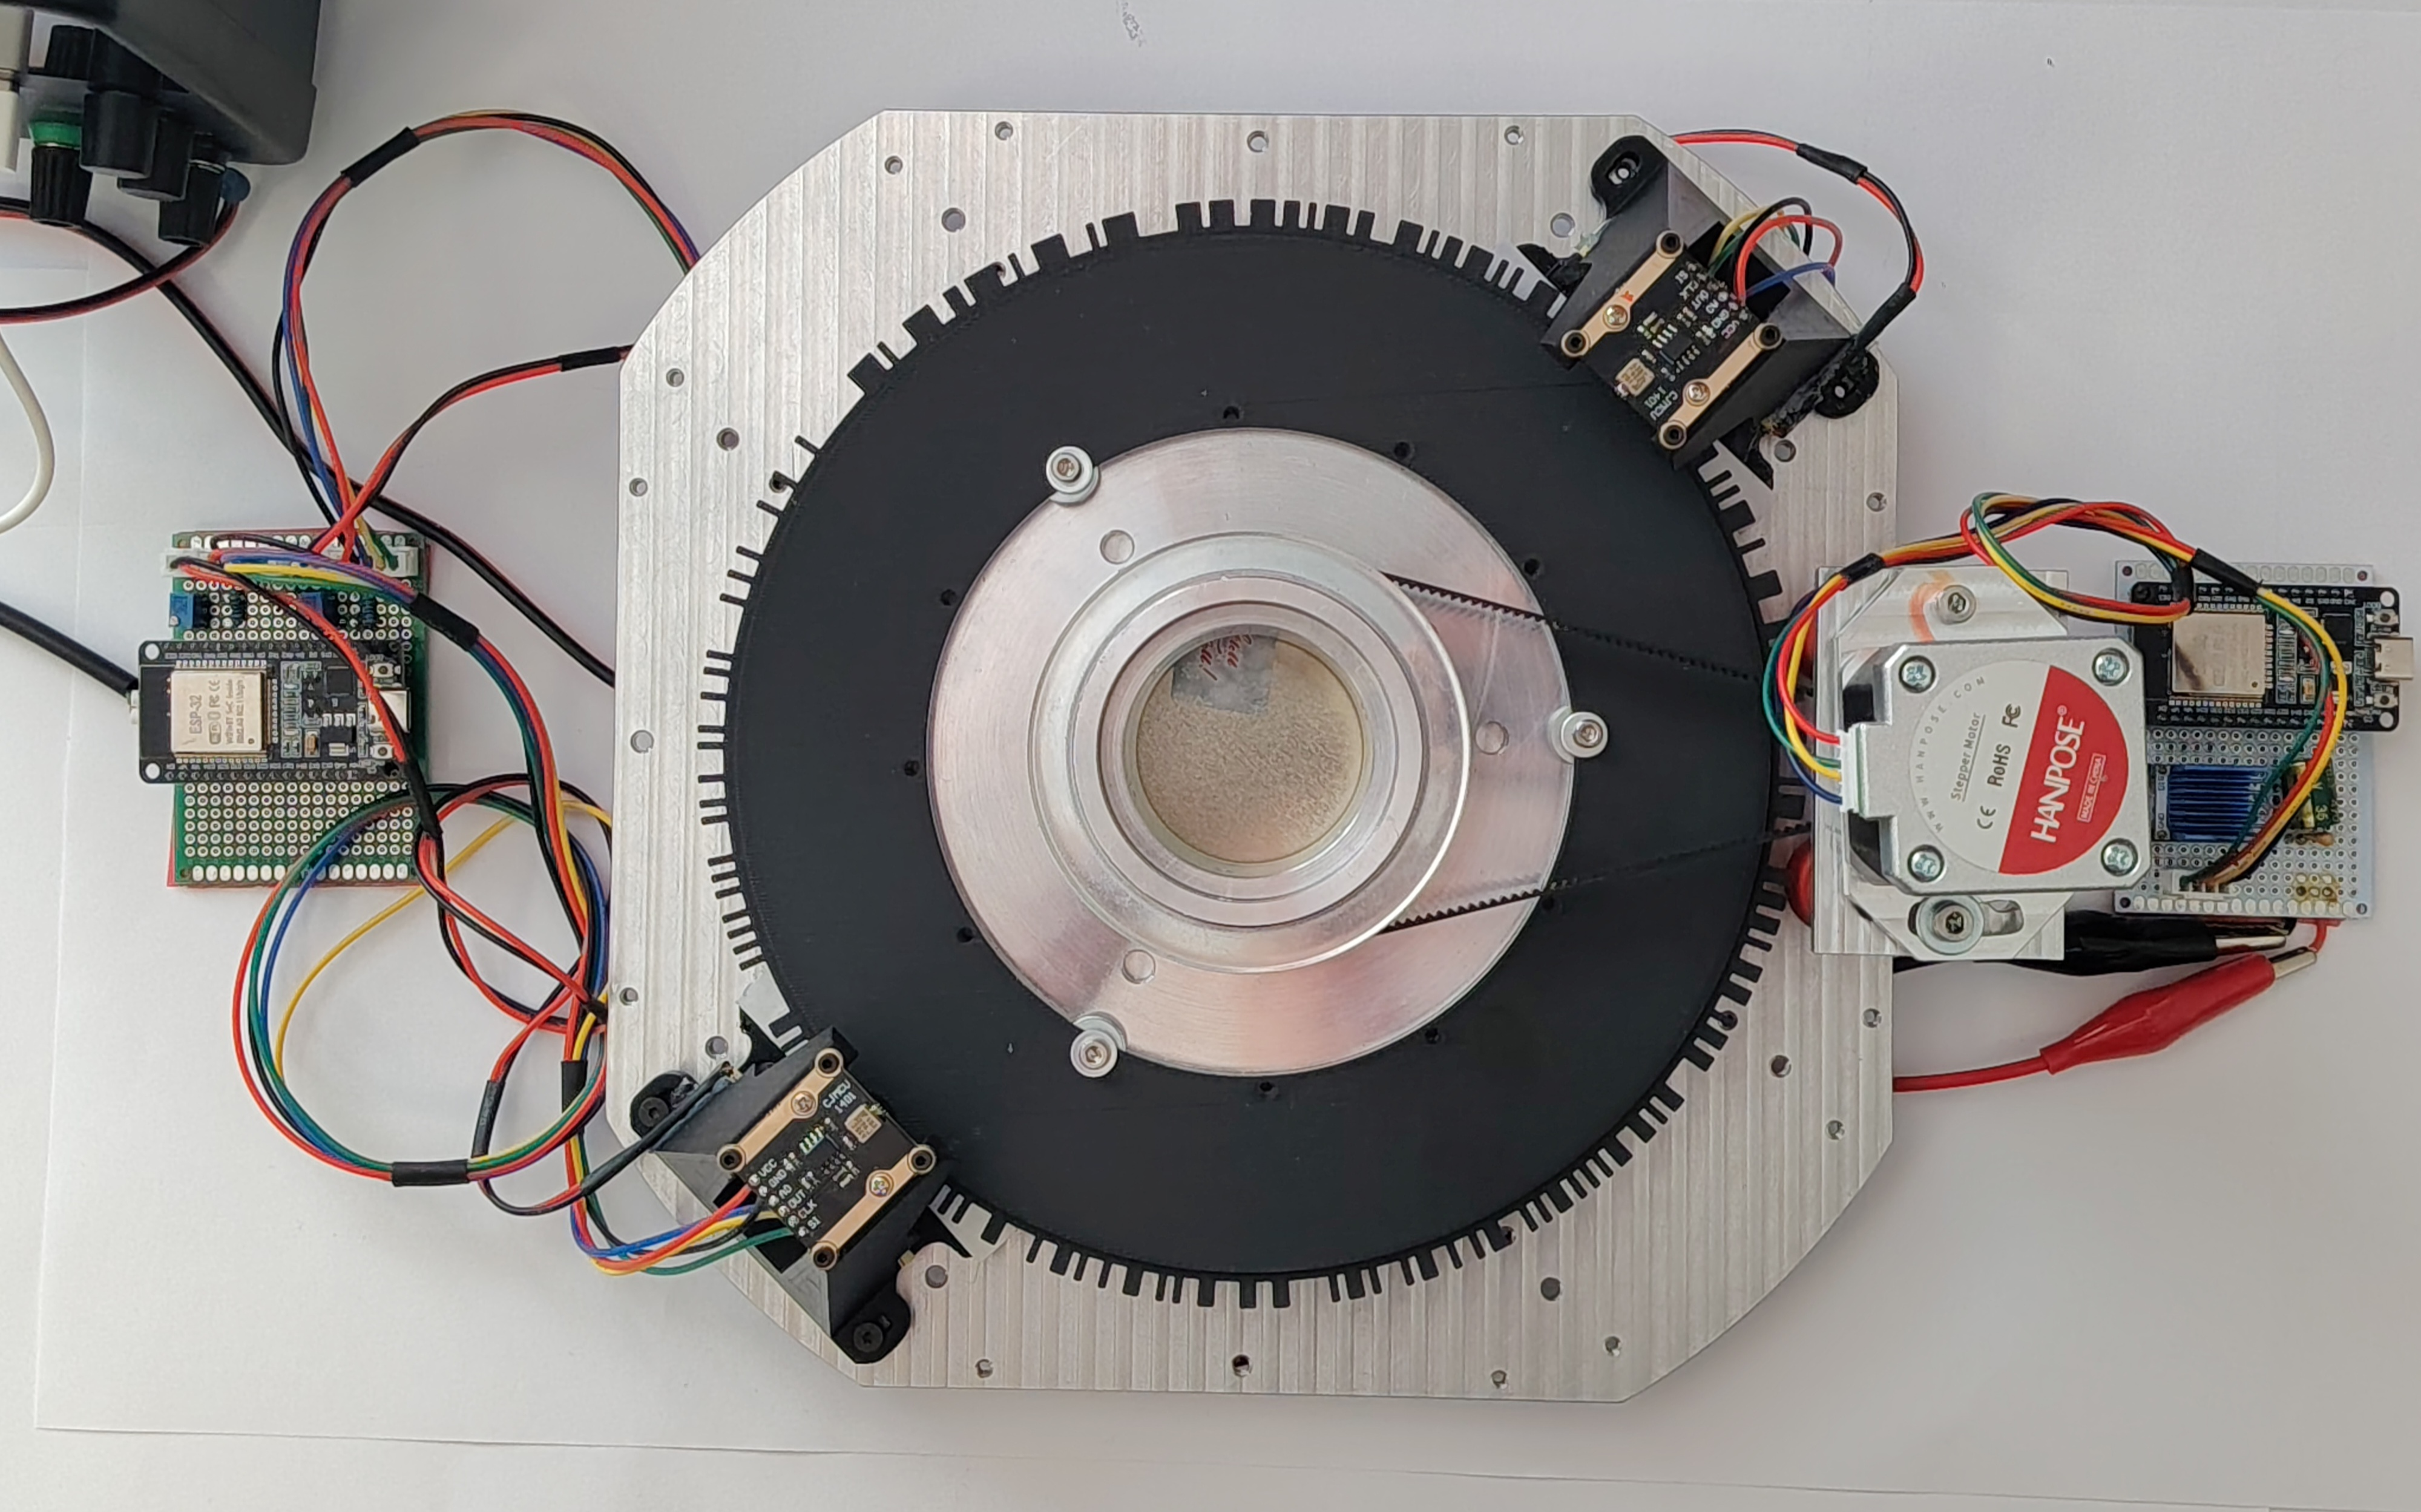
\includegraphics[width=0.9\linewidth]{images/установка две головки.jpg}
    \caption{Фото установки (две головки)}
\end{figure}
\begin{figure}[H]
    \centering
    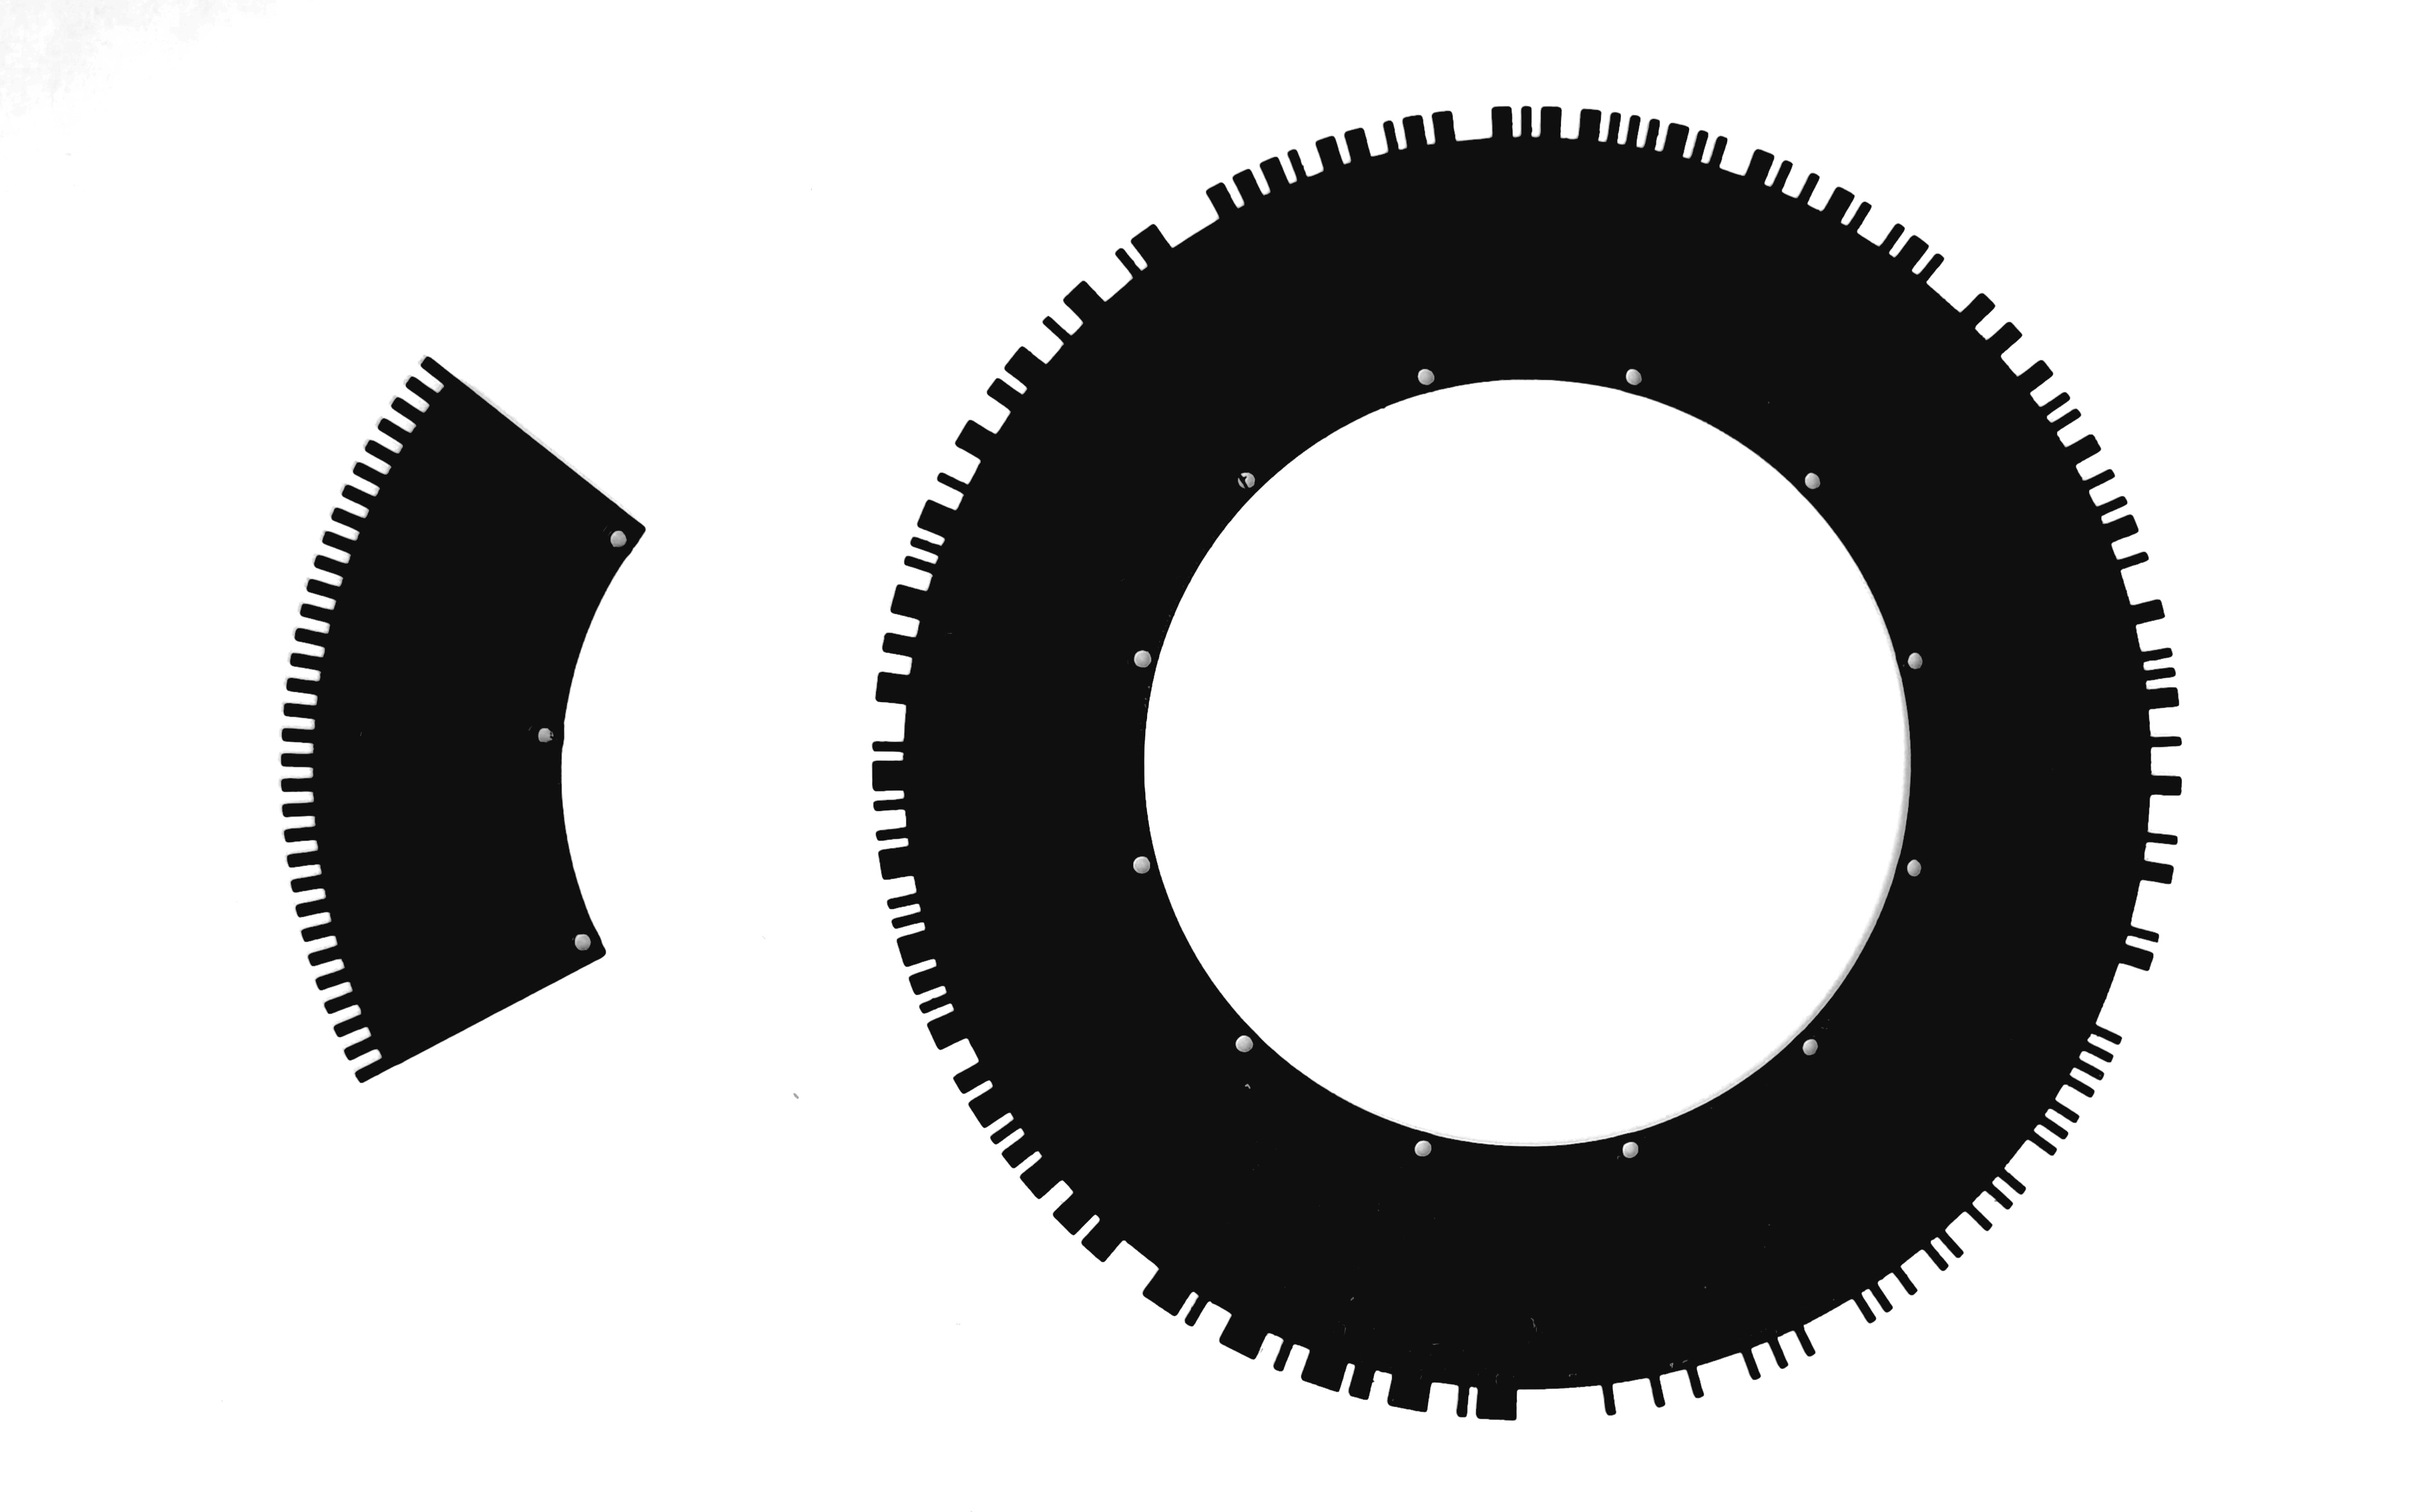
\includegraphics[width=\linewidth]{images/зебра и диск.jpg}
    \caption{Калибровочная <<зебра>> и кодовый диск}
\end{figure}

\subsection{Приложение 2. Демонстрация 3D-модели установки}\label{sec:application2}
\begin{figure}[H]
    \centering
    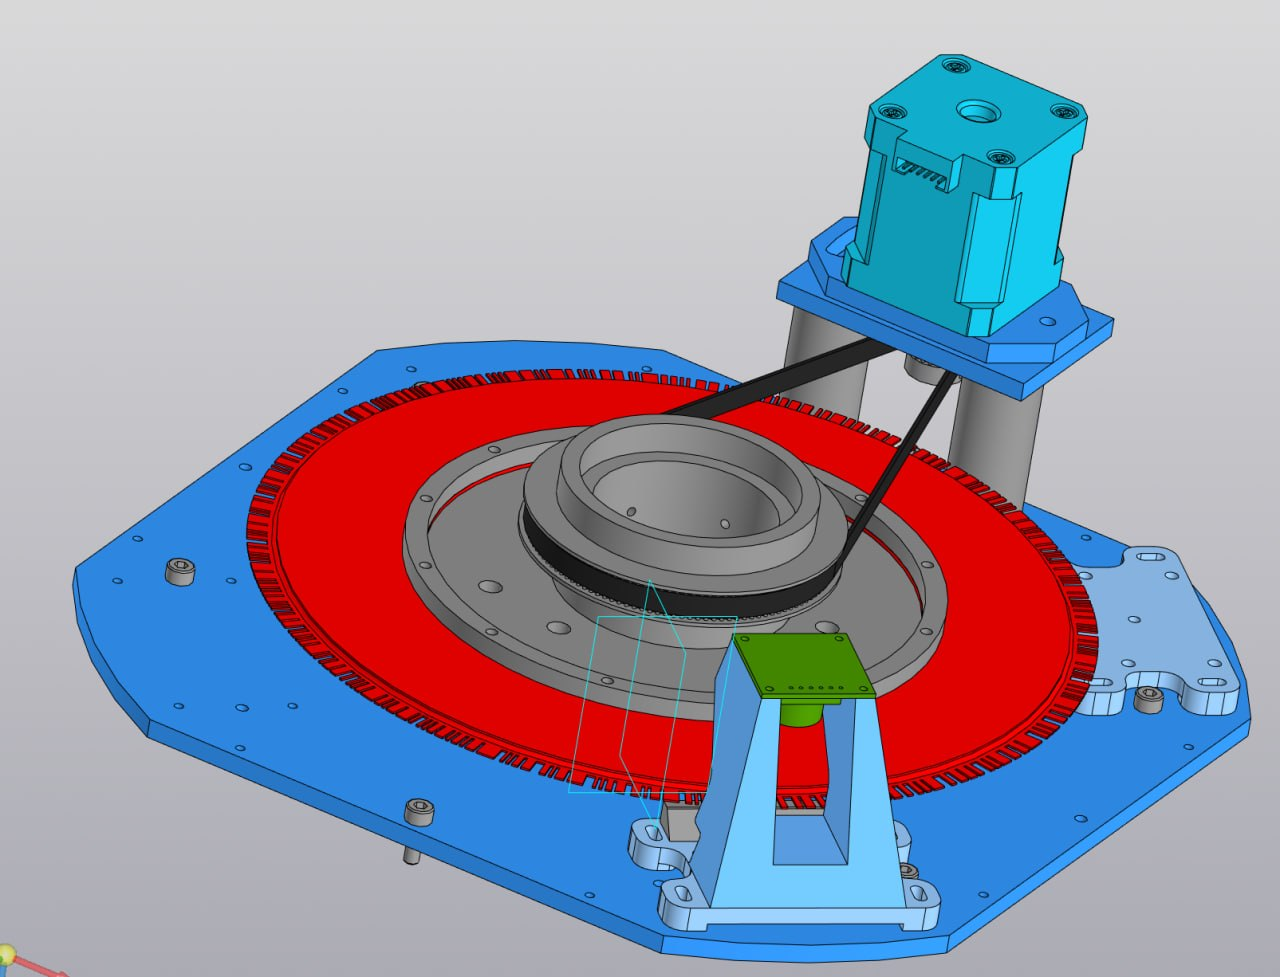
\includegraphics[width=0.9\linewidth]{images/3D модель.png}
    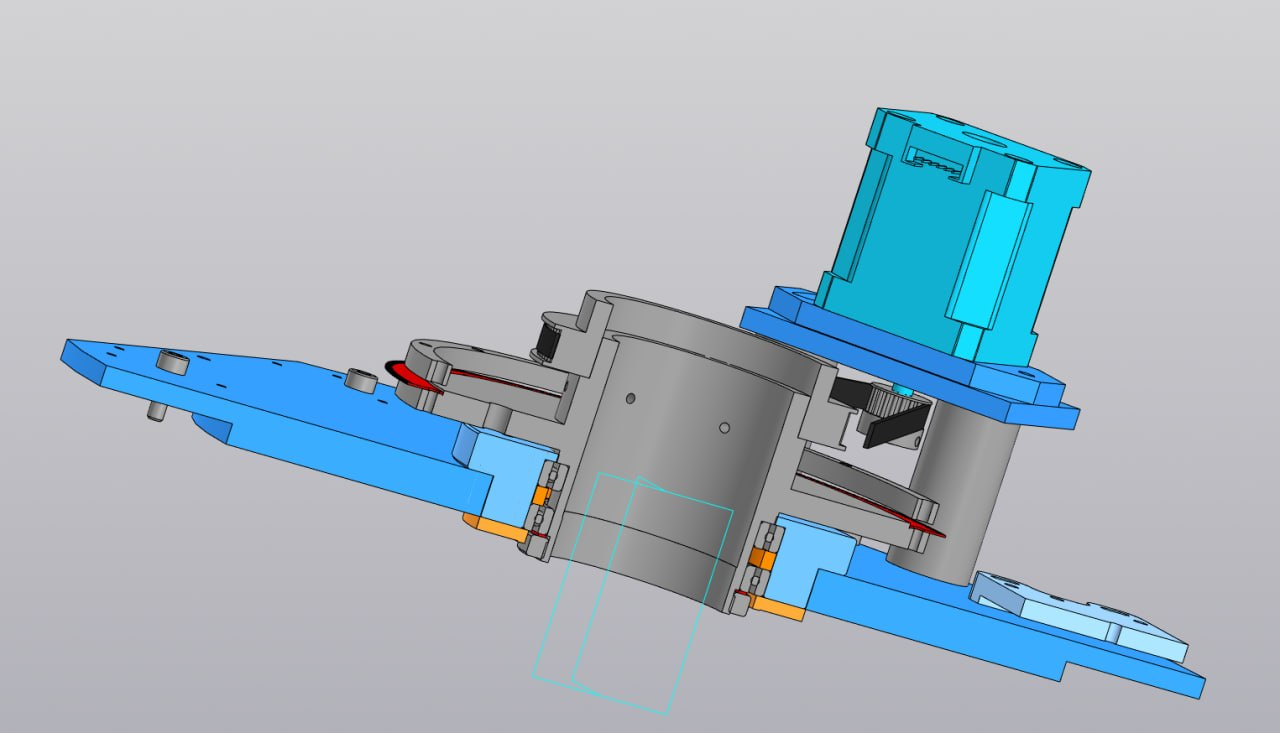
\includegraphics[width=0.9\linewidth]{images/разрез 3D модель.png}
    \caption{3D модель узла энкодера}
\end{figure}

\subsection{Приложение 3. Программный код}
\href{https://github.com/shroomjak/EncoderDecoder.git}{Ссылка на репозиторий}

\subsection{Приложение 4. Диагностические графики точности}\label{sec:application4}
\begin{figure}[H]
\centering
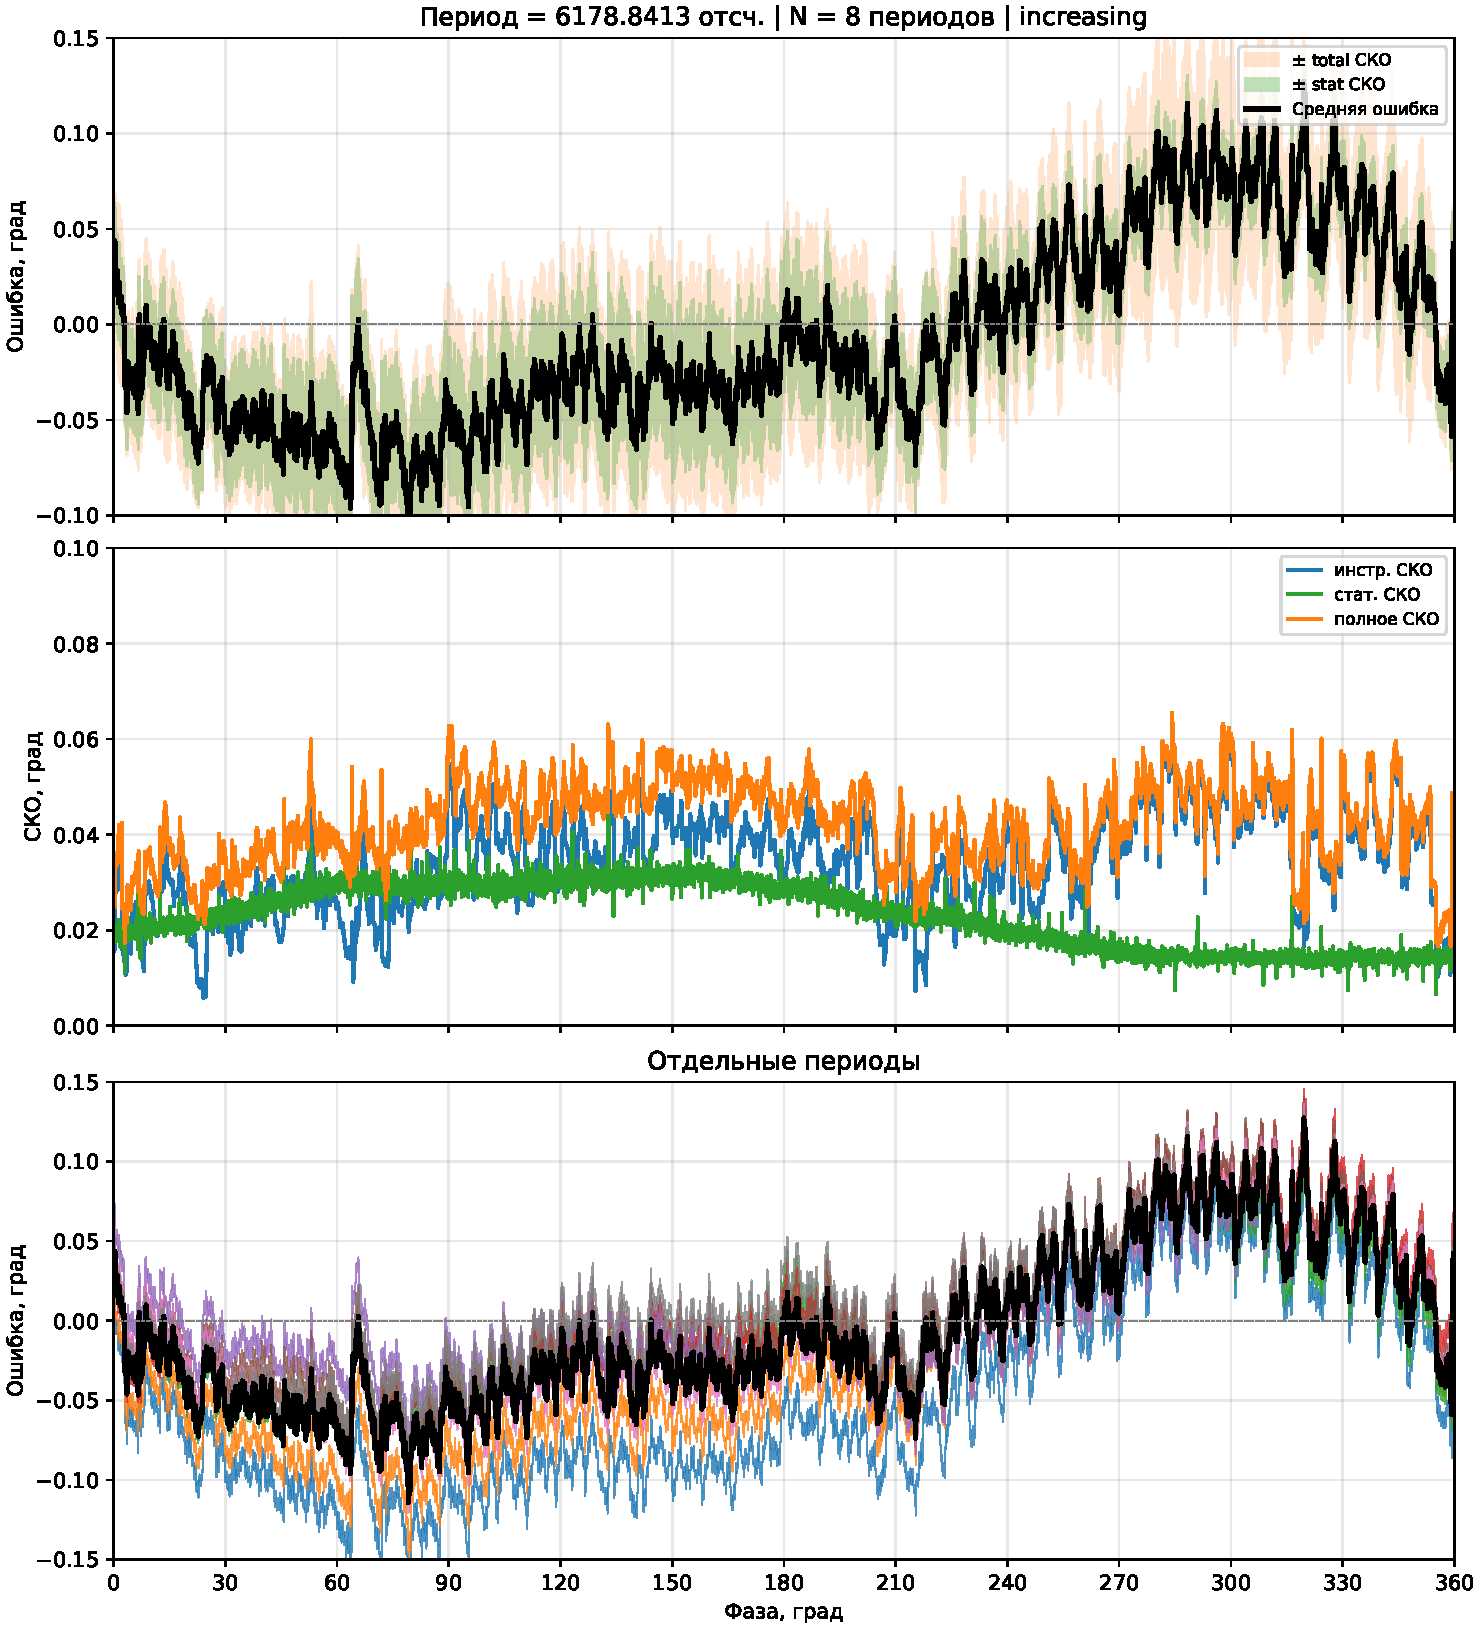
\includegraphics[width=\linewidth]{images/no_trash_2500.pdf}
\caption{Усредненная периодическая ошибка энкодера при скорости 2500 микрошагов в сек. (один оборот за $\sim31$ сек.)}
\label{fig:profile2500}
\end{figure}

\begin{figure}[H]
\centering
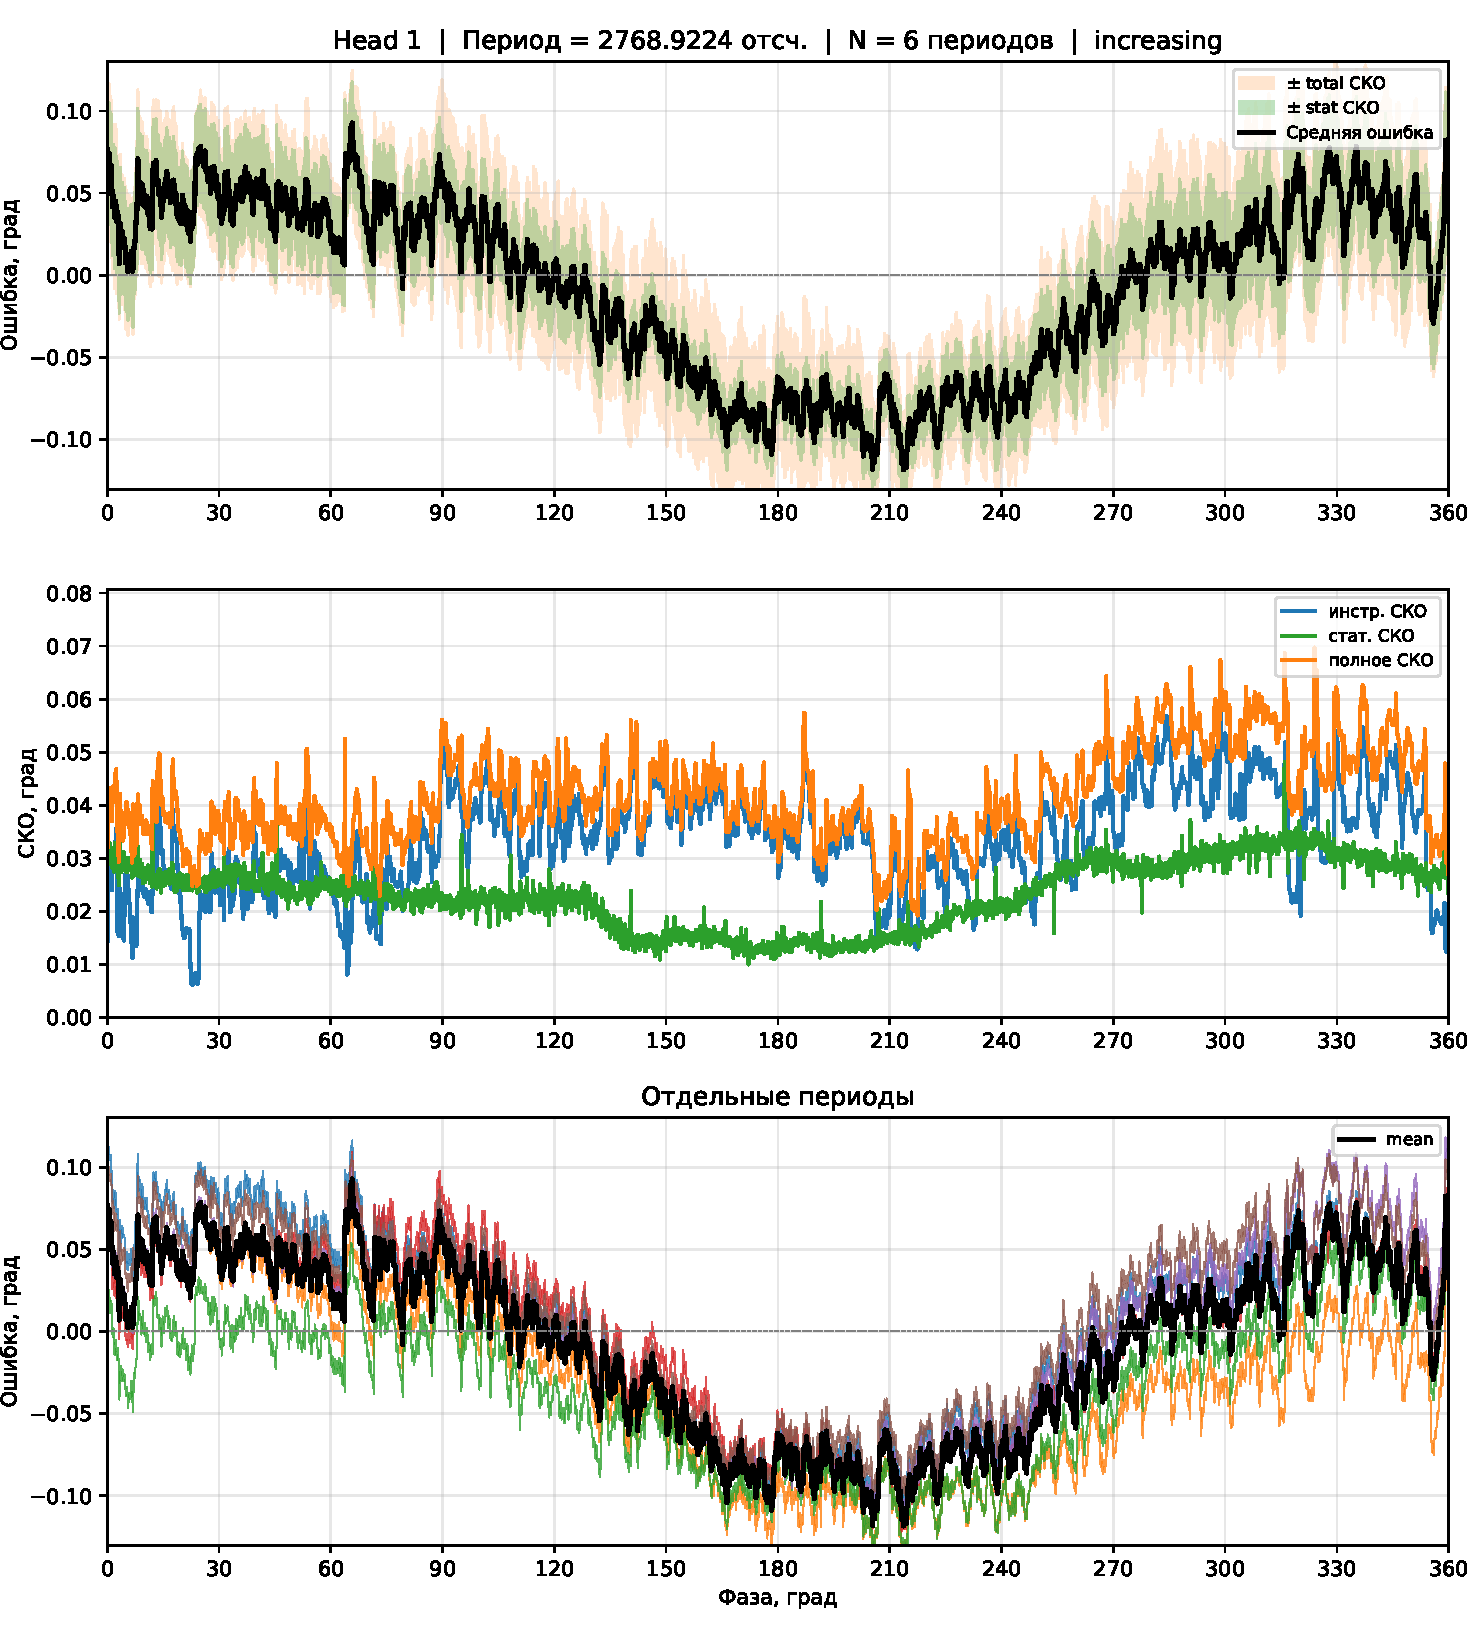
\includegraphics[width=\linewidth]{images/final_10_5000_head1.pdf}
\caption{При скорости 5000 микрошагов в сек. (один оборот за $\sim62$ сек.) с первой головки при вращении согласованно считыванию}
\label{fig:profile5000}
\end{figure}

\begin{figure}[H]
\centering
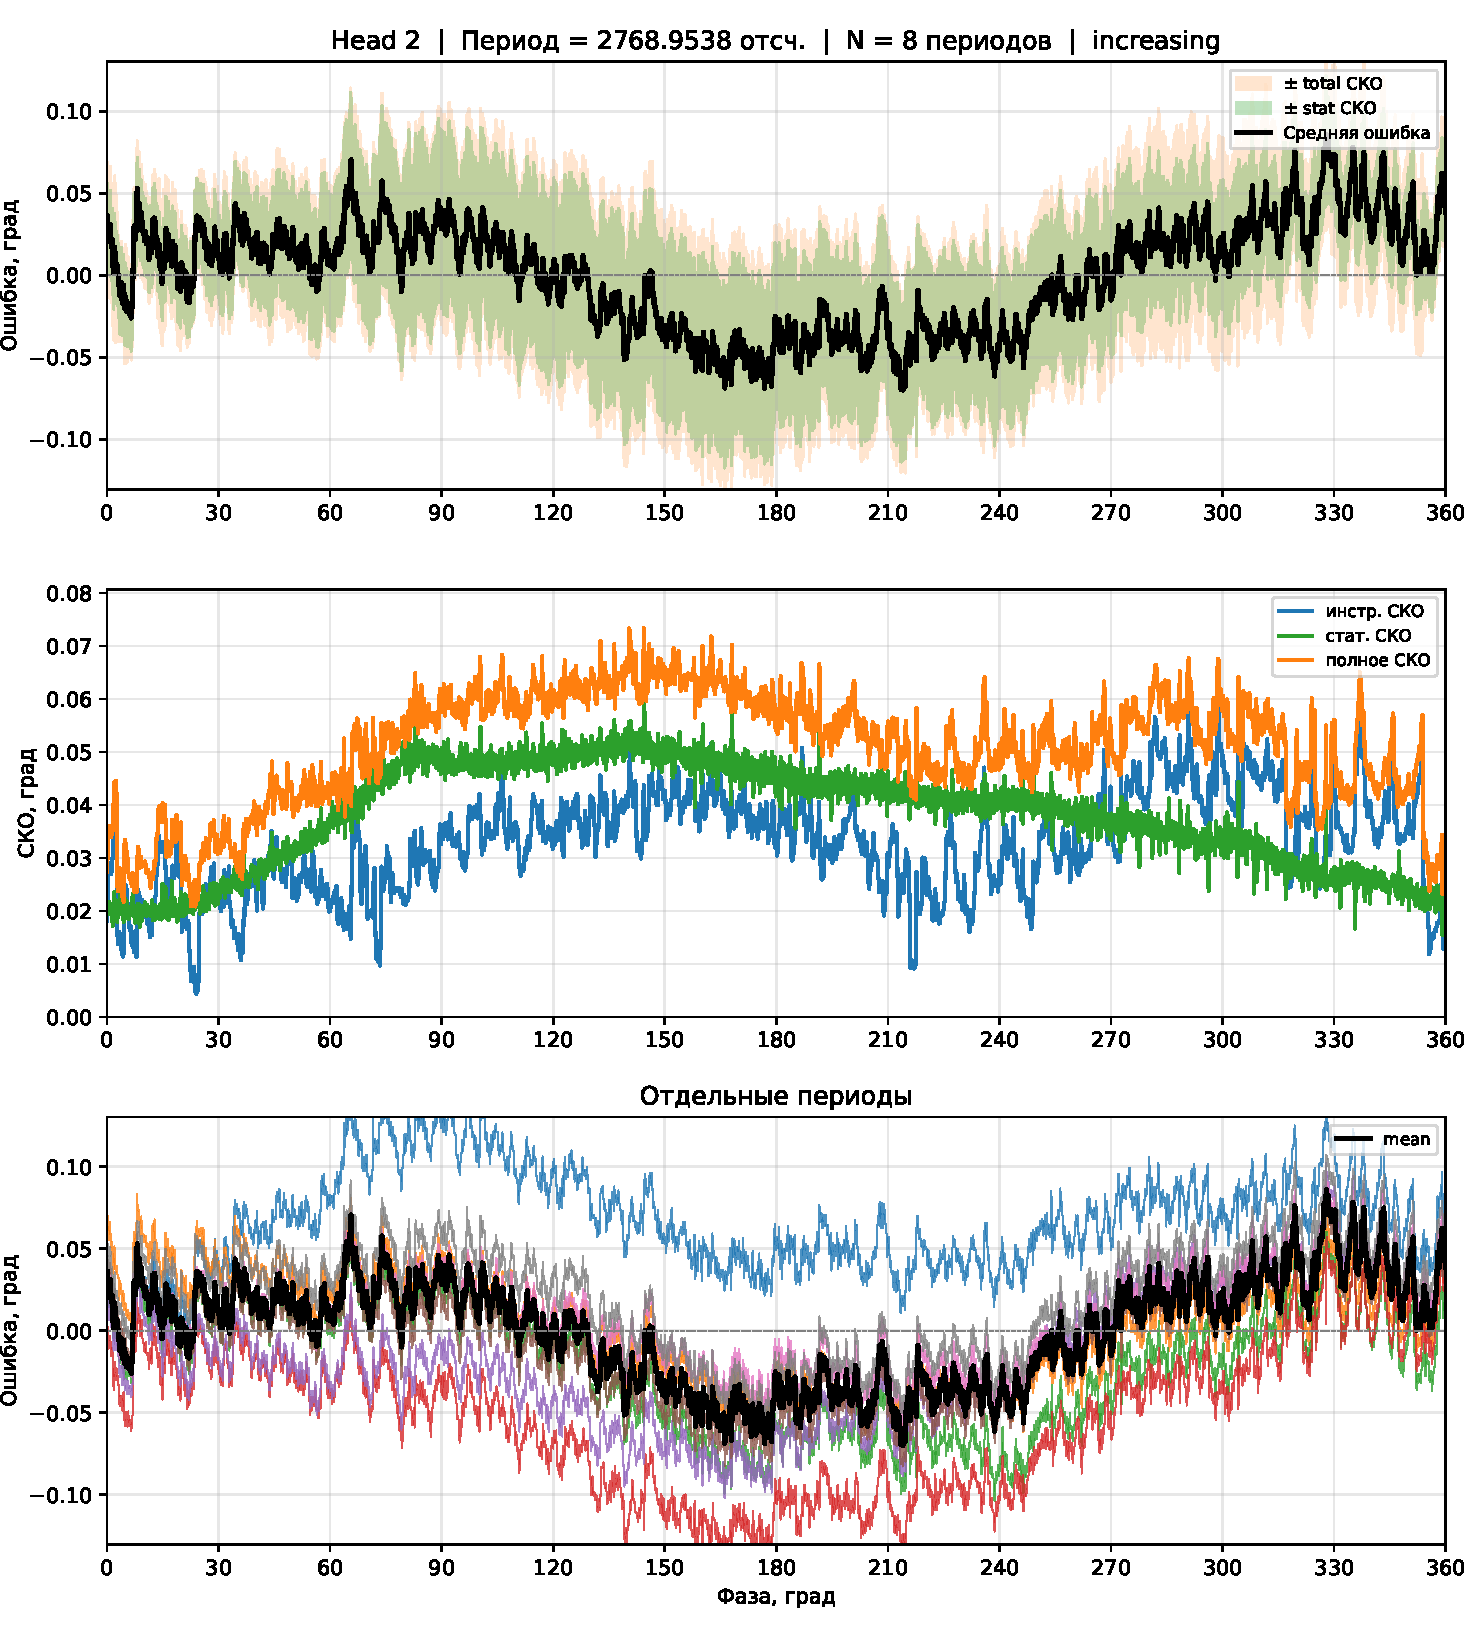
\includegraphics[width=\linewidth]{images/final_10_5000_head2.pdf}
\caption{При скорости 5000 микрошагов в сек. (один оборот за $\sim62$ сек.) со второй головки при вращении согласованно считыванию}
\label{fig:profile5000}
\end{figure}

\begin{figure}[H]
\centering
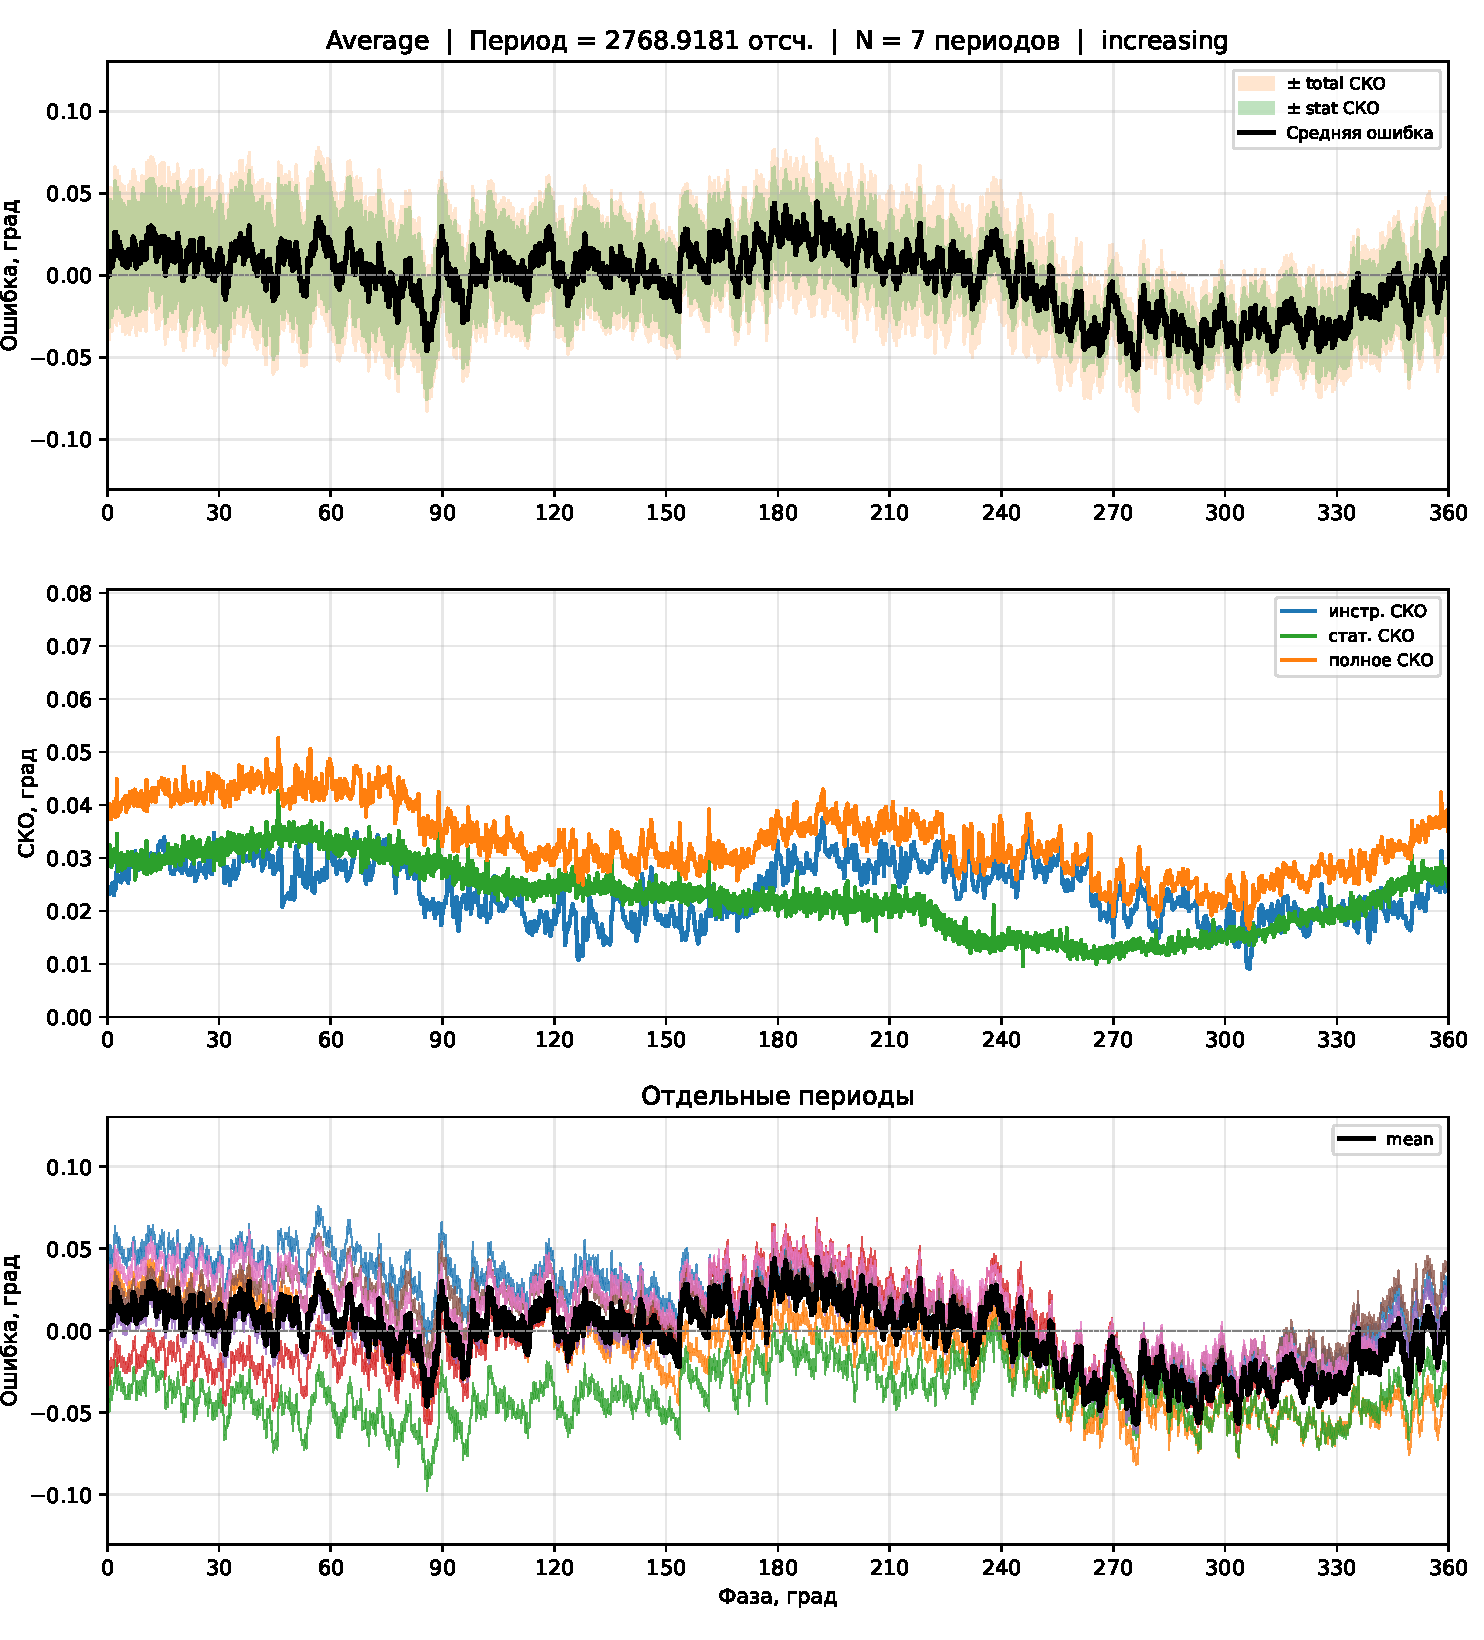
\includegraphics[width=\linewidth]{images/final_10_5000_avg.pdf}
\caption{При скорости 5000 микрошагов в сек. (один оборот за $\sim62$ сек.) круговое среднее показаний двух головок при вращении согласованно считыванию} 
\label{fig:profilerev10000}
\end{figure}

\begin{figure}[H]
\centering
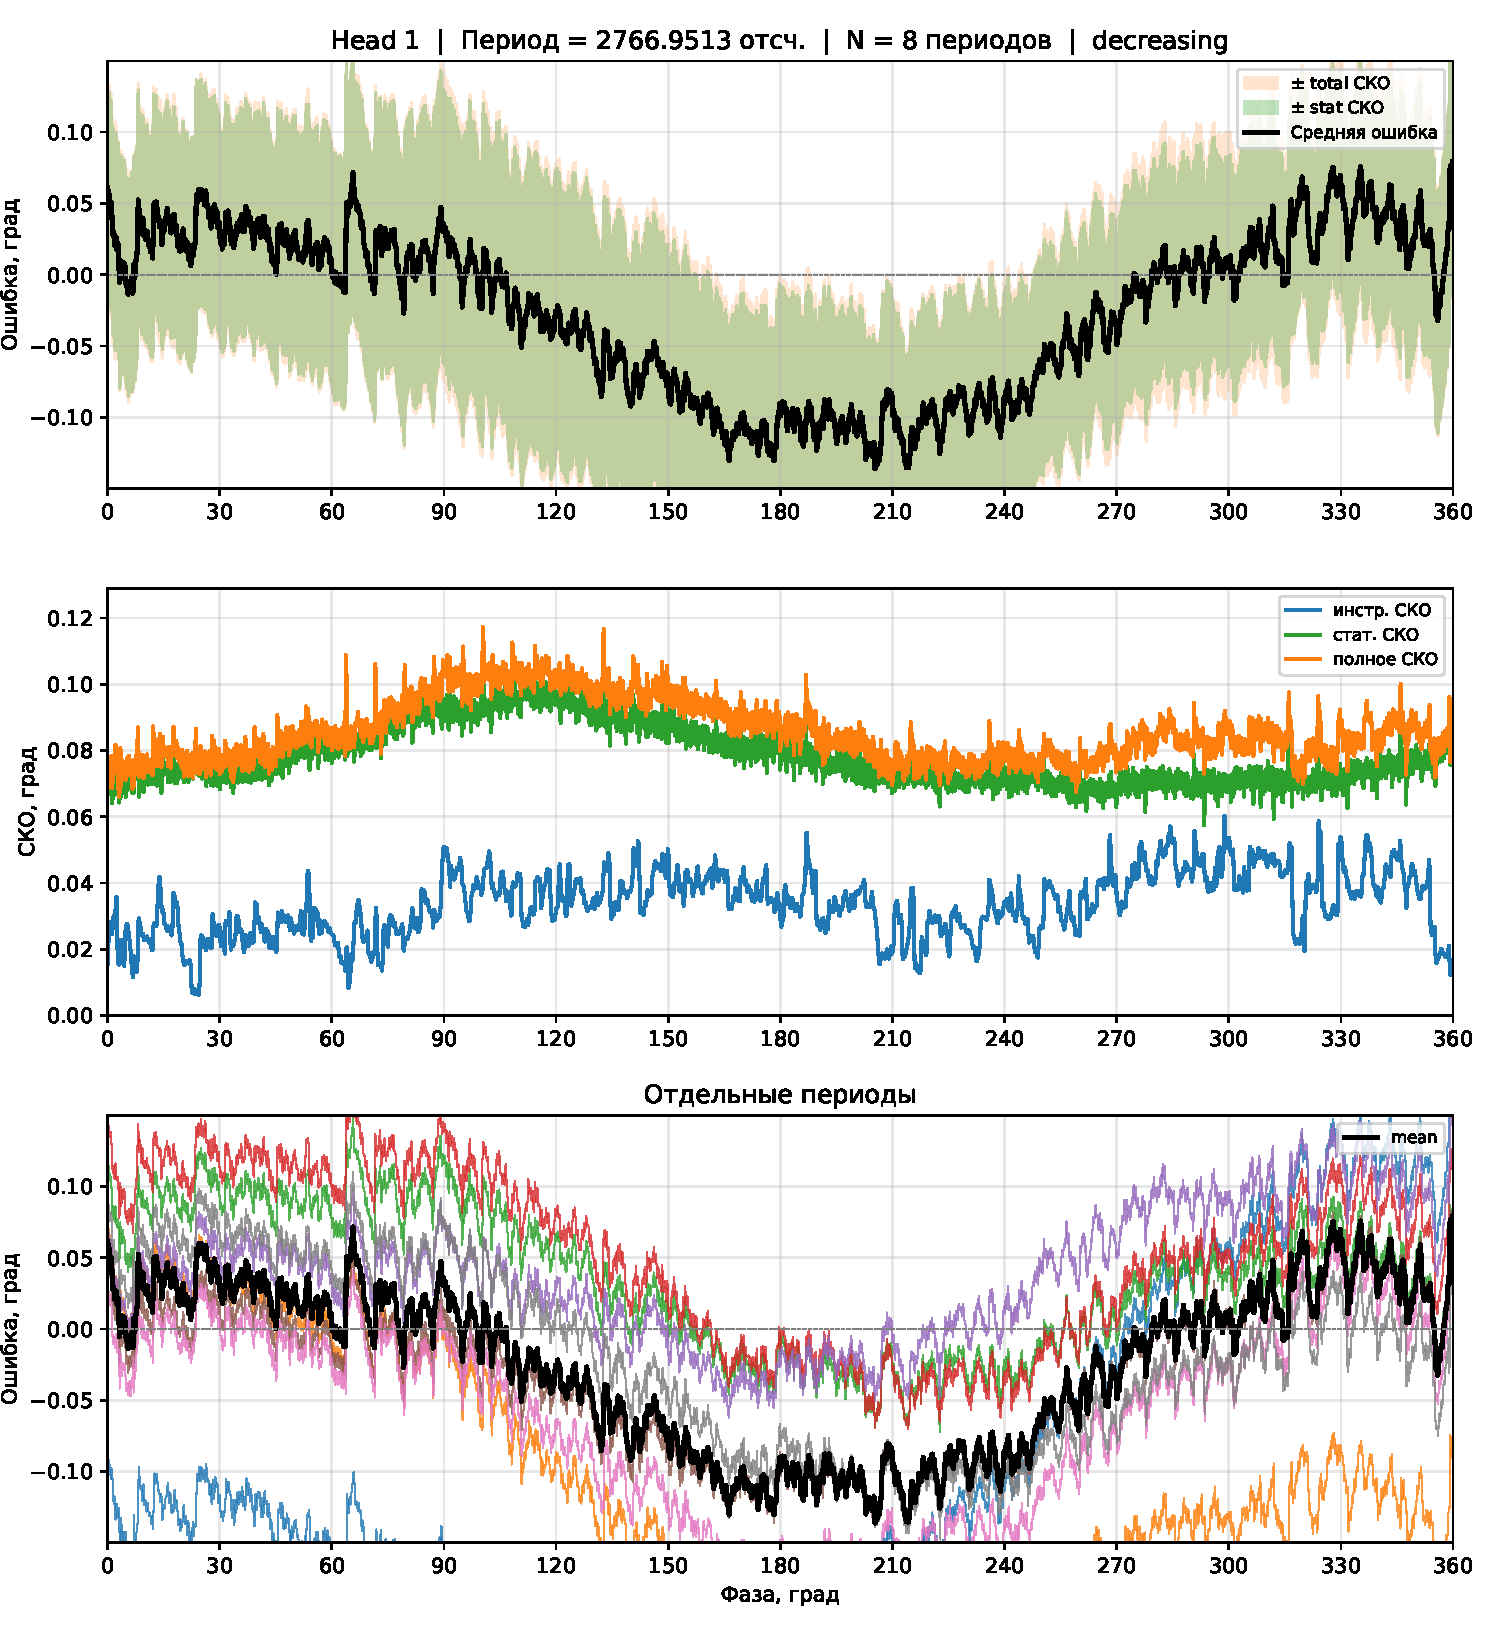
\includegraphics[width=\linewidth]{images/final_reverse10_5000_head1.pdf}
\caption{При скорости 5000 микрошагов в сек. (один оборот за $\sim62$ сек.) с первой головки при вращении противоположно считыванию}
\label{fig:profile5000}
\end{figure}

\begin{figure}[H]
\centering
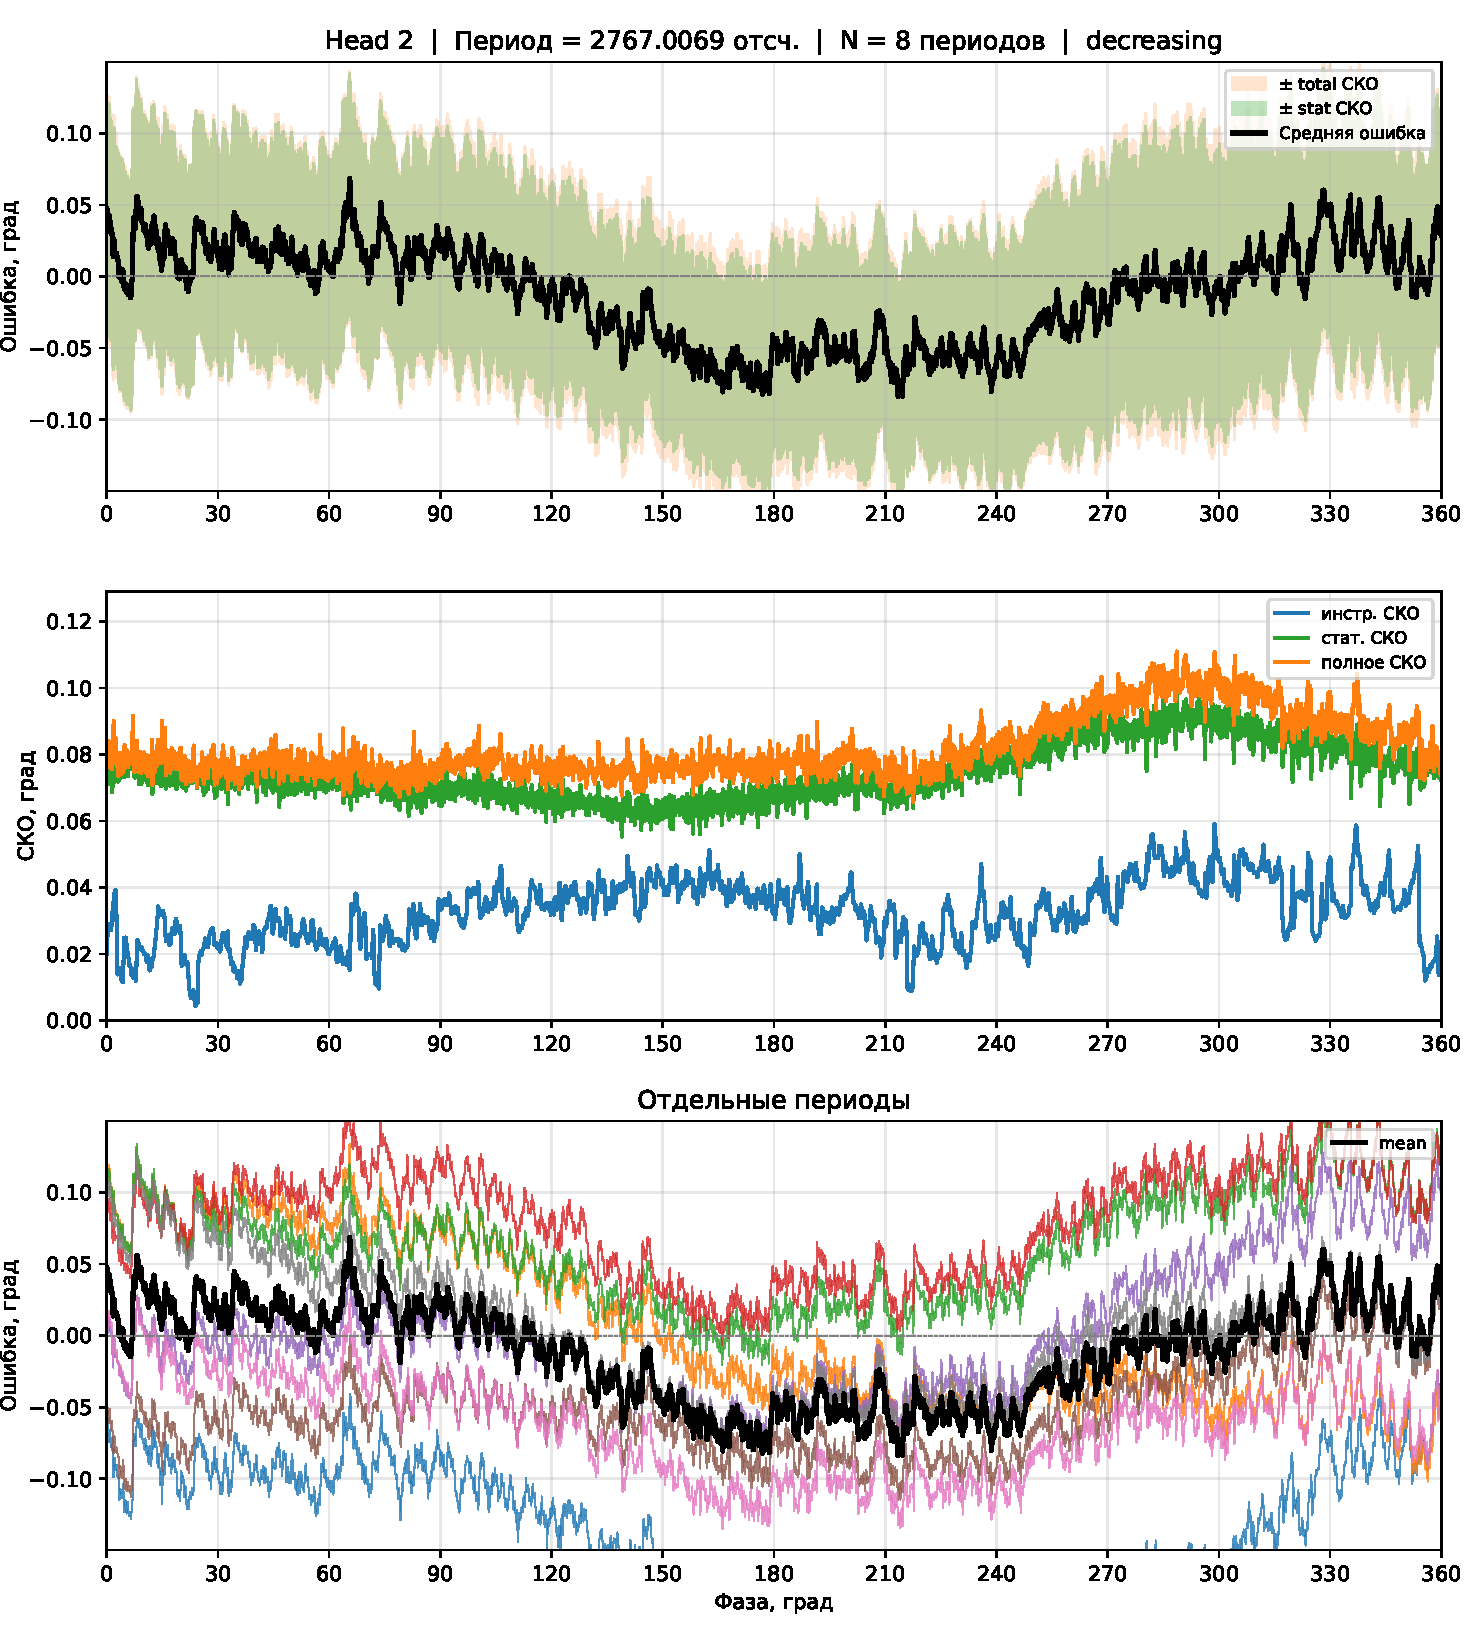
\includegraphics[width=\linewidth]{images/final_reverse10_5000_head2.pdf}
\caption{При скорости 5000 микрошагов в сек. (один оборот за $\sim62$ сек.) со второй головки при вращении противоположно считыванию}
\label{fig:profile5000}
\end{figure}

\begin{figure}[H]
\centering
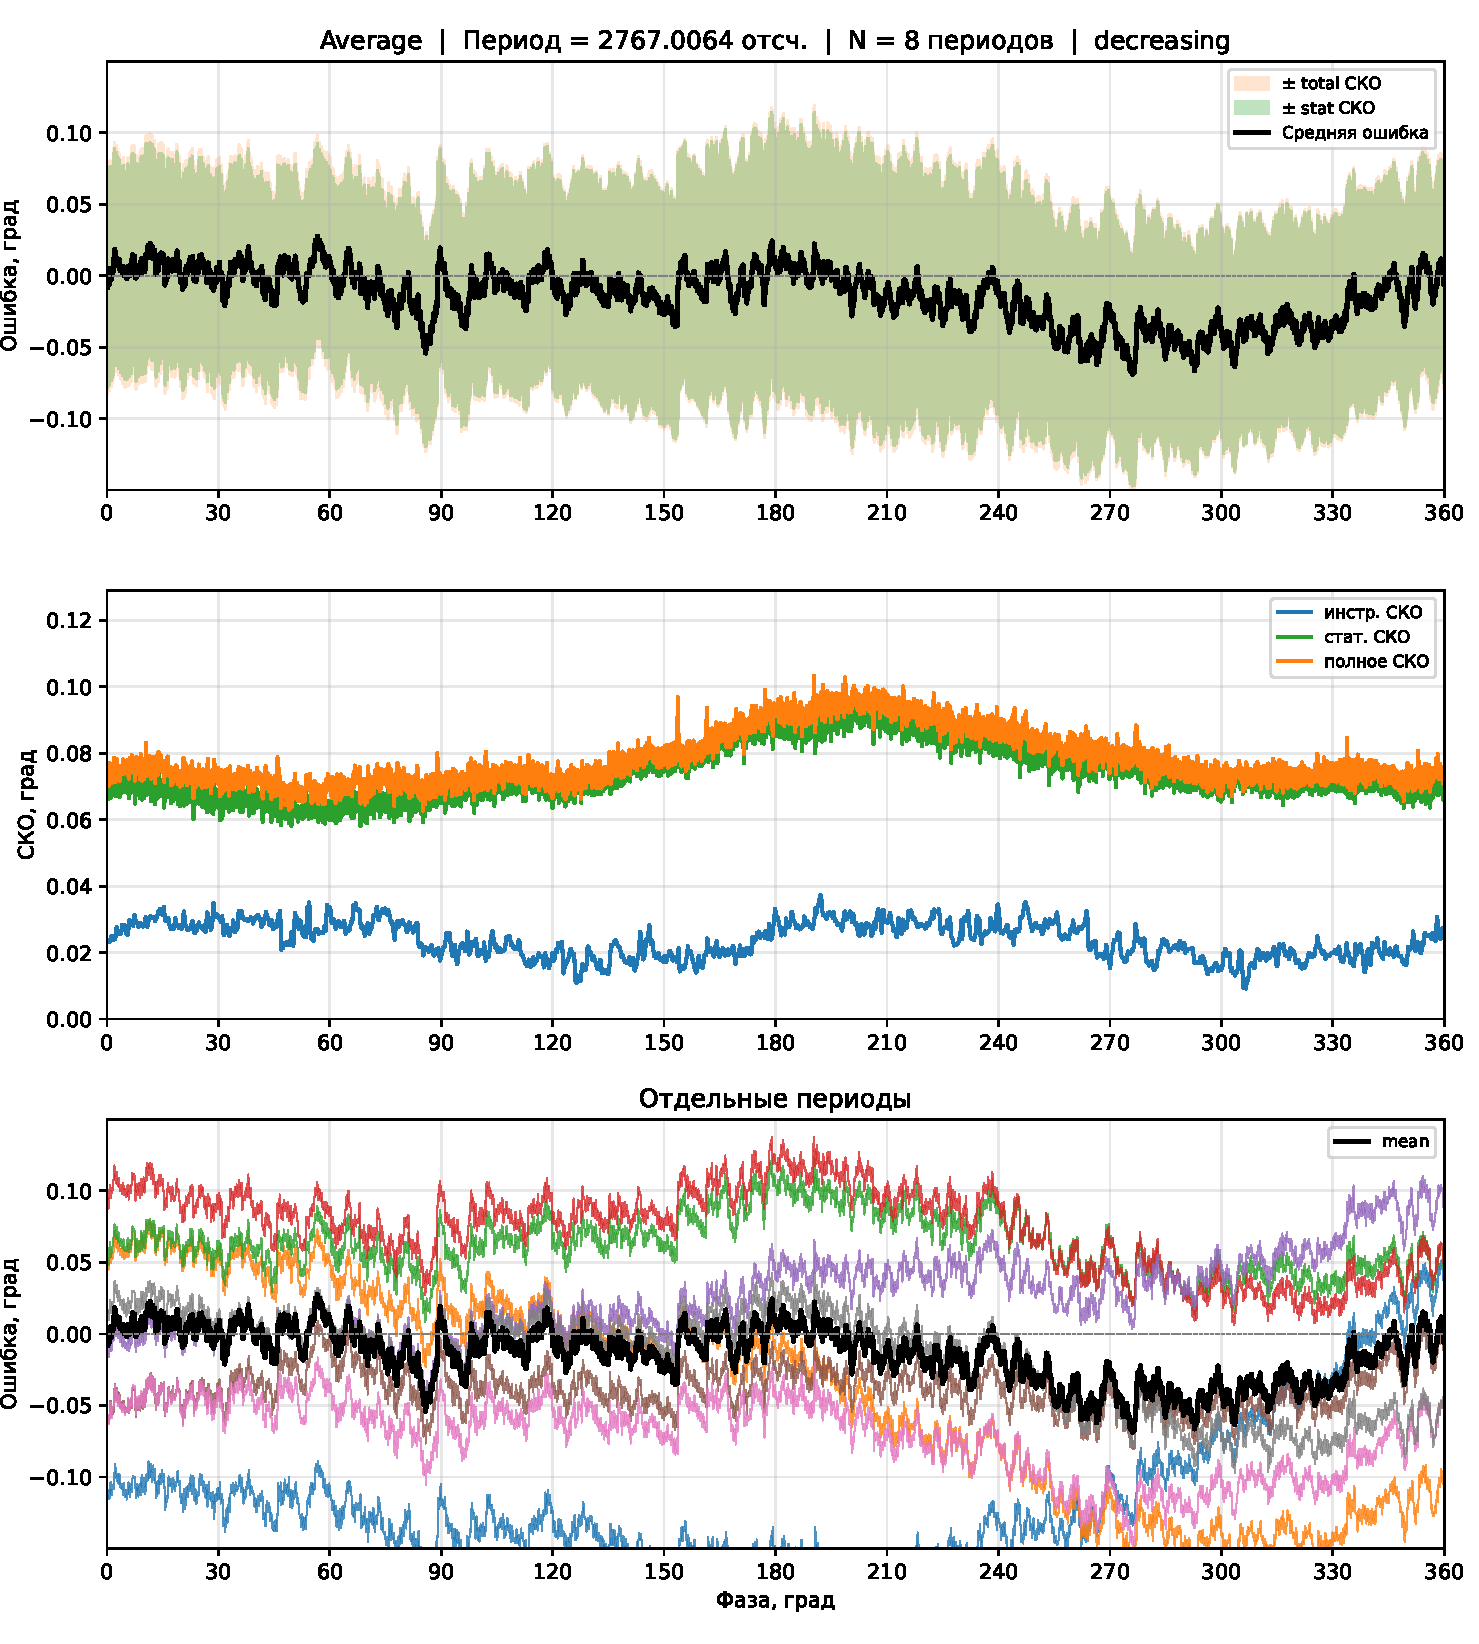
\includegraphics[width=\linewidth]{images/final_reverse10_5000_avg.pdf}
\caption{При скорости 5000 микрошагов в сек. (один оборот за $\sim62$ сек.) круговое среднее показаний двух головок при вращении противоположно считыванию} 
\label{fig:profilerev10000}
\end{figure}




%\pagestyle{empty}

\clearpage
%\bibliographystyle{abbrvnat}
\addcontentsline{toc}{section}{Список литературы}
%\bibliography{lit-base-ru,lit-base-en} %bib файлы вписываем без пробелов
\begin{thebibliography}{99}
\bibitem{dynapar_comm_handbook}
Dynapar.
Encoder Communication Handbook.
Dynapar, Gurnee, IL,
2007.
\url{https://www.dynapar.com/hubfs/uploadedFiles/Downloads/Encoder%20Communications%20Hanbook.pdf}.

\bibitem{renishaw_encoder_accuracy}
Renishaw.
The Accuracy of Rotary Encoders.
\url{https://www.renishaw.com/fr/the-accuracy-of-rotary-encoders--47130}.

\bibitem{gonio}
Y.~V.~Filatov, M.~Y.~Agapov, M.~N.~Bournachev, D.~P.~Loukianov, P.~A.~Pavlov.
Laser goniometer systems for dynamic calibration of optical encoders.
SPIE Optical Metrology,
2003.

\bibitem{24gon}
T.-H.~Hsieh, T.~Watanabe, P.-E.~Hsu.
Calibration of rotary encoders using a shift-angle method.
Applied Sciences,
Volume~12, Issue~10,
Article~5008,
2022.
\url{https://doi.org/10.3390/app12105008}.

\bibitem{polygon}
S.~Kiyono, S.~Zhang, Y.~Uda.
Self-calibration of precision angle sensor and polygon mirror.
Measurement,
Volume~21, Issue~4,
1997,
Pages~125--136,
ISSN~0263-2241,
\url{https://doi.org/10.1016/S0263-2241(97)00054-7}.

\bibitem{table}
M.~H.~Mendenhall, A.~Henins, D.~Windover, J.~P.~Cline.
Characterization of a self-calibrating, high-precision, stacked-stage,
vertical dual-axis goniometer.
Metrologia,
Volume~53, Issue~3,
2016,
Pages~933--944.
\url{https://doi.org/10.1088/0026-1394/53/3/933}.

\bibitem{table_guide}
EURAMET.
Guidelines on the Calibration of Angular Encoders.
EURAMET Calibration Guide No.~23,
Version~1.0 (02/2018).
\url{https://www.euramet.org/Media/news/I-CAL-GUI-023_Calibration_Guide_No._23_web.pdf}.

\bibitem{eccentricity_error}
D.~Gurauskis, D.~Marinkovic, D.~Mažeika, A.~Kilikevičius.
Self-calibratable absolute modular rotary encoder:
development and experimental research.
Micromachines,
Volume~15, Issue~9,
Article~1130,
2024.
\url{https://doi.org/10.3390/mi15091130}.

\bibitem{mpu-ionak}
В.~Ф.~Ионак.
Приборы кинематического контроля.
М.: Машиностроение, 1981.
129~с.

\bibitem{mpu-bachish}
Е.~А.~Бачиш.
Методы воспроизведения единицы плоского угла.
Гироскопия и навигация,
№\,2,
2006,
с.~105--112.

\bibitem{masuda}
T.~Masuda, M.~Kajitani.
An automatic calibration system for angular encoders.
Precision Engineering,
Volume~11, Issue~2,
1989,
Pages~95--100,
ISSN~0141-6359,
\url{https://doi.org/10.1016/0141-6359(89)90043-7}.

\bibitem{watanabe-eda}
T.~Watanabe, H.~Fujimoto, K.~Nakayama, et al.
Automatic high-precision calibration system for angle encoder.
Proc.\ SPIE,
Volume~4401,
2001,
Pages~267--274,
\url{https://doi.org/10.1117/12.424900}.

\bibitem{kiryanov-overview}
В.~П.~Кирьянов, А.~Д.~Петухов, А.~В.~Кирьянов.
Анализ алгоритмов самокалибровки в оптических датчиках угловых перемещений.
Автометрия,
Том~58, №\,3,
2022,
с.~12--23,
\url{https://doi.org/10.15372/AUT20220302}.

\bibitem{cramer}
P.~G.~Cramer.
Mathematical Tools for Analysis, Simulation and Design of Robotic Angular Encoders.
Proceedings of Robotics: Science and Systems,
Ann Arbor, Michigan,
2016,
\url{https://doi.org/10.15607/RSS.2016.XII.028}.

\bibitem{watanabe-selfa}
T.~Watanabe, M.~Kon, N.~Nabeshima, K.~Taniguchi.
An angle encoder for super-high resolution and super-high accuracy using SelfA.
Measurement Science and Technology,
Volume~25, Issue~6,
2014,
Article~065002,
\url{https://doi.org/10.1088/0957-0233/25/6/065002}.

\bibitem{ishii-veda}
T.~Ishii, K.~Taniguchi, K.~Yamazaki, H.~Aoyama.
Development of super-accurate angular encoder system with multi-detecting heads using VEDA method.
Journal of Advanced Mechanical Design, Systems, and Manufacturing,
Volume~12, Number~5,
2018,
Article~JAMDSM0106,
\url{https://doi.org/10.1299/jamdsm.2018jamdsm0106}.

\bibitem{heidenhain-modular-angle-encoders}
DR.~JOHANNES HEIDENHAIN GmbH.
Modular Angle Encoders with Circular Scale.
Technical brochure ID~1401414.
Traunreut, Germany,
\url{https://www.heidenhain.com/fileadmin/pdf/en/01_Products/Prospekte/PR_Modular_Angle_Encoders_Circular_Scale_ID1401414_en.pdf}.

\bibitem{TPoint_Wallace}
P.~T.~Wallace.
TPOINT — Telescope Pointing Analysis System.
Starlink User Note 100.10,
Particle Physics and Astronomy Research Council,
Starlink Project,
9~December~1994.
\url{https://sites.astro.caltech.edu/~srk/TP/Literature/Tpoint_SunWorks.pdf}.

\bibitem{ESO_Horizon}
ESO MIDAS software documentation.
Horizon obstruction tables for equatorial and altazimuth telescopes.
European Southern Observatory, 2003.

\bibitem{ATUS_Stuttgart}
H.~G.~Zoche et al.
The Astronomical Telescope of the University of Stuttgart ATUS:
Mount control and meridian flip management.
University of Stuttgart Observatory technical report, 2017.

\bibitem{EQMOD_Limits}
EQMOD Project.
Setting Limits on Equatorial Mount.
\url{https://eq-mod.sourceforge.net}

\bibitem{EKOS_Flip}
StellarMate / KStars EKOS documentation.
Demystifying the EKOS Automated Meridian Flip.
Main Sequence Software, 2022.

\bibitem{Shatsky2020}
N.~Shatsky, A.~Belinski, A.~Dodin et al.
Caucasian Mountain Observatory of Sternberg Astronomical Institute:
First Six Years of Operation.
\textit{Proc.\ GBAR-2020}, DOI:10.26119/978-5-6045062-0-2\_2020\_127.

\bibitem{EngineersView}
S.~R.~Kulkarni.
Telescope Pointing Errors and Corrections:
an Engineer's View.
Caltech, 2001.
\url{https://sites.astro.caltech.edu/~srk/TP/Literature/EngineersView.pdf}

\bibitem{Renishaw_WP}
Renishaw~plc.
The accuracy of rotary encoders.
White paper, 2017.

\bibitem{Heidenhain_ERA}
Heidenhain GmbH.
Modular Angle Encoders with Circular Scale.
Technical documentation, 2021.
\bibitem{Kiryanov2022}
В.~П.~Кирьянов, А.~Д.~Петухов, А.~В.~Кирьянов.
Анализ алгоритмов самокалибровки в оптических датчиках угловых перемещений.
Автометрия, Т.~58, №\,3, 2022, с.~12--23.
\url{https://doi.org/10.15372/AUT20220302}

\bibitem{singletrack_gray}
F.~Zhang, H.~Zhu, K.~Bian, P.~Liu, J.~Zhang.
Absolute position coding method for angular sensor—single-track Gray codes.
Sensors (Basel),
Volume~18, Issue~8,
2018,
Article~2728.
\url{https://doi.org/10.3390/s18082728}.

\bibitem{mostkom_patent}
А.~А.~Боев, С.~Н.~Кузнецов, А.~А.~Паршин, С.~Ю.~Поляков, С.~Е.~Широбакин.
Способ измерения угла поворота и устройство его реализующее.
Патент RU~2720052~C1,
Опубликовано~23.04.2020,
Заявка~2019127831 от~03.09.2019.

\bibitem{habr_encoder}
Абсолютный поворотный энкодер с однодорожечным кодом Грея [Электронный ресурс] // Хабр, компания RUVDS.
02.12.2021.
URL: \url{https://habr.com/ru/companies/ruvds/articles/592201/} (дата обращения: 09.05.2026).

\bibitem{bahn_vernier}
W.~Bahn, J.~Nam, S.-H.~Lee, D.-I.~Cho.
Digital optoelectrical pulse method for Vernier-type rotary encoders.
IEEE Transactions on Instrumentation and Measurement,
Volume~65,
2016,
Pages~431--440.

\bibitem{blais_rioux_peak}
F.~Blais, M.~Rioux.
Real-time numerical peak detector.
Signal Processing,
Volume~11, Issue~2,
1986,
Pages~145--155.

\bibitem{debruijn_cutdown}
J.~Sawada.
Cut-down de Bruijn sequences.
Online resource,
\url{http://debruijnsequence.org/db/cutdown},
Last accessed: 12.05.2026.

\bibitem{steger_subpixel}
C.~Steger.
Analytical and empirical performance evaluation of subpixel line and edge detection.
In: K.~J.~Bowyer, P.~J.~Phillips (eds.),
Empirical Evaluation Methods in Computer Vision.
World Scientific,
1998.
\url{https://mv.in.tum.de/_media/members/steger/publications/1998/eemcv-98-steger.pdf}.

\bibitem{gioi_canny_devernay}
R.~Grompone~von~Gioi, G.~Randall.
A sub-pixel edge detector: an implementation of the Canny/Devernay algorithm.
Image Processing On Line,
Volume~7,
2017,
Pages~347--372.
\url{https://doi.org/10.5201/ipol.2017.216}.


\bibitem{phase_matching_sampling}
Z.~Mou, K.~Zhu, L.~Zheng, Y.~Fang, J.~Mou, C.~Jiang.
Phase matching sampling algorithm for sampling rate reduction in TDM interferometric sensor arrays.
Opto-Electronic Technology,
Volume~1, Issue~2,
2025,
Article~250006.
\url{https://doi.org/10.29026/oet.2025.250006}.

\bibitem{aleman_lens_distortion}
M.~Alemán\mbox{-}Flores, L.~Alvarez, L.~Gomez, D.~Santana\mbox{-}Cedrés.
Automatic lens distortion correction using one-parameter division models.
Image Processing On Line,
Volume~4,
2014,
Pages~327--343.
\url{https://doi.org/10.5201/ipol.2014.106}.

\end{thebibliography}
\end{document}
